\documentclass[pdftex,letterpaper,12pt]{report}
\usepackage{thesis}
\usepackage{amsmath}
\usepackage{amssymb}
\usepackage{amsthm}
\usepackage{mathtools}
\usepackage{bm}
\usepackage{gensymb}
\usepackage{wasysym}
\usepackage{mathtools}
\usepackage{physics}
\usepackage{empheq}
\usepackage{cases}
\usepackage{rotating}
\usepackage{subfig}
\usepackage{caption}
\usepackage{multirow}
\captionsetup{labelfont=bf} 
\captionsetup[subfloat]{position=top,singlelinecheck=off,justification=raggedright,font=bf,labelfont=large,labelformat=simple,captionskip=-2mm}
\usepackage{float}
\usepackage{enumitem} 
\usepackage[toc,page]{appendix}






\begin{document}
	
\begin{subequations}\label{InitialSpinup}
	\begin{gather}
	P_{pc}(t)=\gamma_{se}P_{A}t-\frac{1}{2}\gamma_{se}P_{A}(\gamma_{se}+\Gamma_{pc}+d_{pc})t^{2}\\
	P_{tc}(t)=\frac{1}{2}\gamma_{se}P_{A}d_{tc}t^{2}
	\end{gather}
\end{subequations}

\begin{equation}
k_{se}^{K}=(7.46\pm 0.62)\times 10^{-20}cm^{3}/s
\end{equation}

The Faraday rotation angle $\phi_{r}$ is

\begin{table*}\scriptsize
	\begin{center}
		\begin{tabular}{|c|c|ccc|ccc|ccccc|cc|c|}
			\hline
			\multirow{2}{*}{\begin{sideways}{EXP}\end{sideways}}&\multirow{2}{*}{Cell} & \multirow{2}{*}{Lasers} & $I_0$ & T$_\mathrm{pc}^\mathrm{set}$ & \multirow{2}{*}{$P_\mathrm{He}^\infty$} & $\Gamma_\mathrm{s}^{-1}$ & $\langle\Gamma\rangle^{-1}$ & \multirow{2}{*}{$\langle P^\mathrm{A} \rangle$} & \multirow{2}{*}{$P_\mathrm{line}^\mathrm{A}$} & \multirow{2}{*}{$D_\mathrm{fr}$} & \multirow{2}{*}{$D_\mathrm{pb}$} & [Rb]$_\mathrm{fr}$ & $\Delta$T$_\mathrm{Rb}$ & $\Delta$T$_\mathrm{He}$ & \multirow{2}{*}{X}\\
			&& & W/cm$^2$ & $^\circ$C & & hrs & hrs & & & & & $10^{14}$/cm$^3$ & $^\circ$C & $^\circ$C &\\
			\hline
			\hline
			\multirow{5}{*}{\begin{sideways}saGDH\end{sideways}} & Proteus & 3B & 3.8 & 180 & 0.46 & 27 & 74 & - & - & 0 & 0 & - & - & - & -\\
			\cline{2-16}
			& Priapus & 3B & 3.8 & 180 & 0.44 & 21 & 56 & - & - & 0 & 0 & - & - & - & -\\
			\cline{2-16}
			& Penelope & 3B & 3.8 & 180 & 0.39 & 18 & 46 & - & - & 0 & 0 & - & - & - & -\\
			\cline{2-16}
			& Powell & 3B & 3.8 & 180 & 0.38 & 13 & 25 & - & - & 0 & 0 & - & - & - & -\\
			\cline{2-16}
			& Prasch & 3B & 3.8 & 180 & 0.33 & 13 & 33 & - & - & 0 & 0 & - & - & - & -\\
			\hline
			\hline
			\multirow{20}{*}{\begin{sideways}GEN\end{sideways}} & \multirow{2}{*}{Al} & 2.5B & 3.2 & 235 & 0.53(04) & 7.86(08) & 24.2(9) & - & - & 20* & 4.53(25) & - & - & - & - \\
			& & 5B & 6.1 & 235 & 0.54(04) & 6.73(21) & 24.2(9) & - & - & 20* & 4.53(25) & - & - & - & - \\
			\cline{2-16}
			& \multirow{2}{*}{Barbara} & 2.5B & 1.6 & 235 & 0.37(03) & 5.5(08) & 38.8(1.6) & - & - & 20* & 4.80(25) & - & - & - & - \\
			& & 5B & 3.1 & 235 & 0.57(04) & 4.76(63) & 38.8(1.6) & - & - & 20* & 4.80(25) & - & - & - & - \\
			\cline{2-16}
			& Gloria & 3B & 1.7 & 235 & 0.60(04) & 6.13(06) & 31.6(1.5) & - & - & 20* & 7.20(40) & - & - & - & - \\
			\cline{2-16}
			& \multirow{2}{*}{Anna} & 1B & 0.6 & 235 & 0.33(02) & 5.60(36) & 9.50(71) & - & - & 20* & 9.64(57) & - & - & - & - \\
			& & 1.5B & 1.0 & 235 & 0.39(02) & 5.37(16) & 9.50(66) & - & - & 20* & 9.50(71) & - & - & - & - \\
			\cline{2-16}
			& \multirow{2}{*}{Dexter} & 1.5B & 1.5 & 235 & 0.47(04) & 7.58(17) & 16.5(7) & - & - & 20* & 20* & - & - & - & - \\
			& & 5B & 6.1 & 235 & 0.49(04) & 6.63(13) & 16.5(7) & - & - & 20* & 20* & - & - & - & - \\
			\cline{2-16}
			& Edna & 3B & 2.4 & 235 & 0.56(04) & 5.71(02) & 26.5(1.5) & - & - & 5* & 3.63(20) & - & - & - & - \\
			\cline{2-16}
			& \multirow{2}{*}{Dolly} & 3B & 1.0 & 235 & 0.43(03) & 6.16(07) & 30.3(1.5) & - & - & 20* & 20(1.3) & - & - & - & - \\
			& & 1N1B & 1.4 & 235 & 0.62(03) & 5.79(07) & 30.2(1.6) & - & - & 20* & 20(1.3) & - & - & 16(10) & - \\
			\cline{2-16}
			& \multirow{3}{*}{Simone} & 2N1B & 3.8 & 215 & 0.32(02) & 14.1(1) & 20.0(7) & 0.90(13)  & 0.91(05) & 10.7(5) & 8.89(45) & 0.20(03) & -7(13) & - & -0.04(11)$^\star$ \\
			& & 2N1B & 3.8 & 240 & 0.48(04) & 6.89(20) & 19.9(8) & - & - & - & 9.76(49) & - & - & - & - \\
			& & 2N1B & 3.8 & 255 & 0.58(03) & 6.05(13) & 19.9(8) & 0.90(13) & 0.92(05) & 12.5(8) & 10.3(52) & 0.90(12) & -4(4) & - & 0.14(13)$^\star$ \\
			\cline{2-16}
			& \multirow{5}{*}{Sosa} & 2N1B & 1.9 & 160 & 0.57(03) & 16.7(09) & 57.0(5) & 0.91(14) & 1.00(03) & 0 & 0 & 1.97(26) & 4(1) & 30(7) & 0.17(10)$^\dagger$ \\
			&  & 2N1B & 1.9 & 170 & 0.61(03) & 11.7(03) & 56.8(7) & 0.90(12) & 0.98(03) & 0 & 0 & 3.0(6) & 3(4) & 38(14) & 0.21(15)$^\star$ \\
			&  & 2N1B & 1.9 & 180 & 0.55(03) & 8.79(09) & 56.6(9) & 0.87(14) & 0.97(03) & 0 & 0 & 4.30(89) & 1(5) & 47(7) & 0.38(11)$^\dagger$ \\
			&  & 2N1B & 1.9 & 190 & 0.40(03) & 6.39(22) & 56.2(1.2) & 0.72(18) & 0.82(03) & 0 & 0 & 5.72(1.61) & -2(6) & 48(20) & 0.55(30)$^\star$ \\
			&  & 2N1B & 1.9 & 200 & 0.26(01) & 5.04(17) & 56.1(1.3) & - & - & 0 & 0 & - & - & ? & - \\
			%& 2C1F & 1.9 & 160 & 0.57(03) & 16.7(09) & 55.7(1.8) & 1.00(03) & 0 & 0 & -\\
			% & 2C1F & 1.9 & 170 & 0.61(03) & 11.7(03) & 55.5(2.0) & 0.98(03) & 0 & 0 & -\\
			% & 2C1F & 1.9 & 180 & 0.55(03) & 8.79(09) & 55.2(2.2) & 0.97(03) & 0 & 0 & - \\
			% & 2C1F & 1.9 & 190 & 0.40(02) & 6.39(22) & 55.1(2.3) & - & 0 & 0 & -\\
			% & 2C1F & 1.9 & 200 & 0.26(01) & 5.40(17) & 55.4(2.1) & 0.83(17) & 0 & 0 & -\\
			\hline
			\hline
			\multirow{12}{*}{\begin{sideways}Transversity\end{sideways}} & Boris & 3B & 1.8 & 235 & 0.42(03) & 6.25(06) & 21.1(1.2) & 0.69(21) & 0.79(07) & 1.96(18) & 2.45(23) & 2.19(61) & -8(5) & - & 0.36(14)$^\star$ \\
			\cline{2-16}
			& \multirow{2}{*}{Samantha} & 3B & 1.8 & 235 & 0.50(03) & 6.30(13) & 20.9(1.1) & - & - & 5* & 4.34(23) & - & - & - & -\\
			& & 3N & 2.6 & 235 & 0.68(03) & 4.62(03) & 17.2(1.0) & 0.96(04) & 0.99(03) & 4.37(10) & 4.34(23) & 1.80(24) & 7(2) & 21(10) & 0.11(07)$^\star$\\
			\cline{2-16}
			& Alex & 2N1B & 2.6 & 235 & 0.59(03) & 4.81(03) & 27.2(1.6) & 0.92(10) & 0.99(03) & 1.37(08) & 1.19(07) & 4.08(56) & 0(6) & 42(10) & 0.38(10)$^\dagger$ \\
			\cline{2-16}
			& Moss & 1N1B & 1.8 & 235 & 0.62(03) & 5.35(04) & 24.6(1.4) & 0.93(12) & 0.95(09) & 5* & 2.40(13) & - & - & 29(8) & 0.20(16)$^\S$\\
			\cline{2-16}
			& Tigger & 1N1B & 1.8 & 235 & 0.51(03) & 4.89(05) & 12.2(8) & 0.97(11) & 0.95(09) & 5* & 5* & - & - & 23(9) & 0.18(16)$^\S$\\
			\cline{2-16}
			& Astral Weeks & 2N1B & 2.6 & 235 & 0.69(03) & 6.57(12) & 35.6(1.6) & 0.99(04) & 0.99(03) & 7.09(55) & 6.21(56) & 0.97(16) & 3(5) & 25(4) & 0.22(05)$^\dagger$\\
			\cline{2-16}
			& Stephanie & 3N & 2.6 & 235 & 0.71(04) & 4.55(09) & 37.3(2.0) & 0.93(09) & 0.99(03) & 1.39(11) & 1.50(10) & 5.08(91) & 7(8) & 54(6) & 0.18(12)$^\star$\\
			\cline{2-16}
			& \multirow{3}{*}{Brady} & 1N & 0.9 & 235 & 0.62(03) & 4.8(1.1) & 27.1(1.6) & - & 0.95(03) & 5* & 2.36(24) & -  & - & 14(9) & -\\
			& & 2N & 1.8 & 235 & 0.68(03) & 5.52(70) & 27.2(1.5) & - & 0.99(03) & 5* & 2.36(24) & - & - & 25(8) & -\\
			& & 3N & 2.6 & 235 & 0.70(03) & 5.30(01) & 27.2(1.4) & 0.93(09) & 0.99(03) & 2.60(20) & 2.36(24) & 2.87(54) & 6(7) & 39(9) & 0.12(07)$^\dagger$\\
			\cline{2-16}
			& Maureen & 3N & 2.6 & 235 & 0.66(03) & 5.42(12) & 23.5(1.3) & 0.97(11) & 0.97(09) & 5* & 4.42(55) & - & - & - & 0.16(15)$^\S$\\
			\hline
		\end{tabular}
	\end{center}
	\caption{Cell Performance for three sets of experiments: saGDH (top), GEN (middle), and Transversity (bottom).  Within each experiment grouping, data is sorted by type of laser used (B = Broadband, N = Narrowband).  *Indicates nominal value for $D$.  $^\S$ indicates X was attained using spinup and alkali polarization data, $^\star$ indicates X was also measured using faraday rotation, $^\dagger$ indicates X was also measured using the early-time behavior of the spinup.}
	\label{table:CellTable}
\end{table*}

The coefficients of pressure broadening for $^{3}$He, $^{4}$He and N$_{2}$ are listed in Table~\ref{PBCoef}.

\begin{figure}[H]
	\label{spinup}
	\centering
	\resizebox{0.91\textwidth}{!}{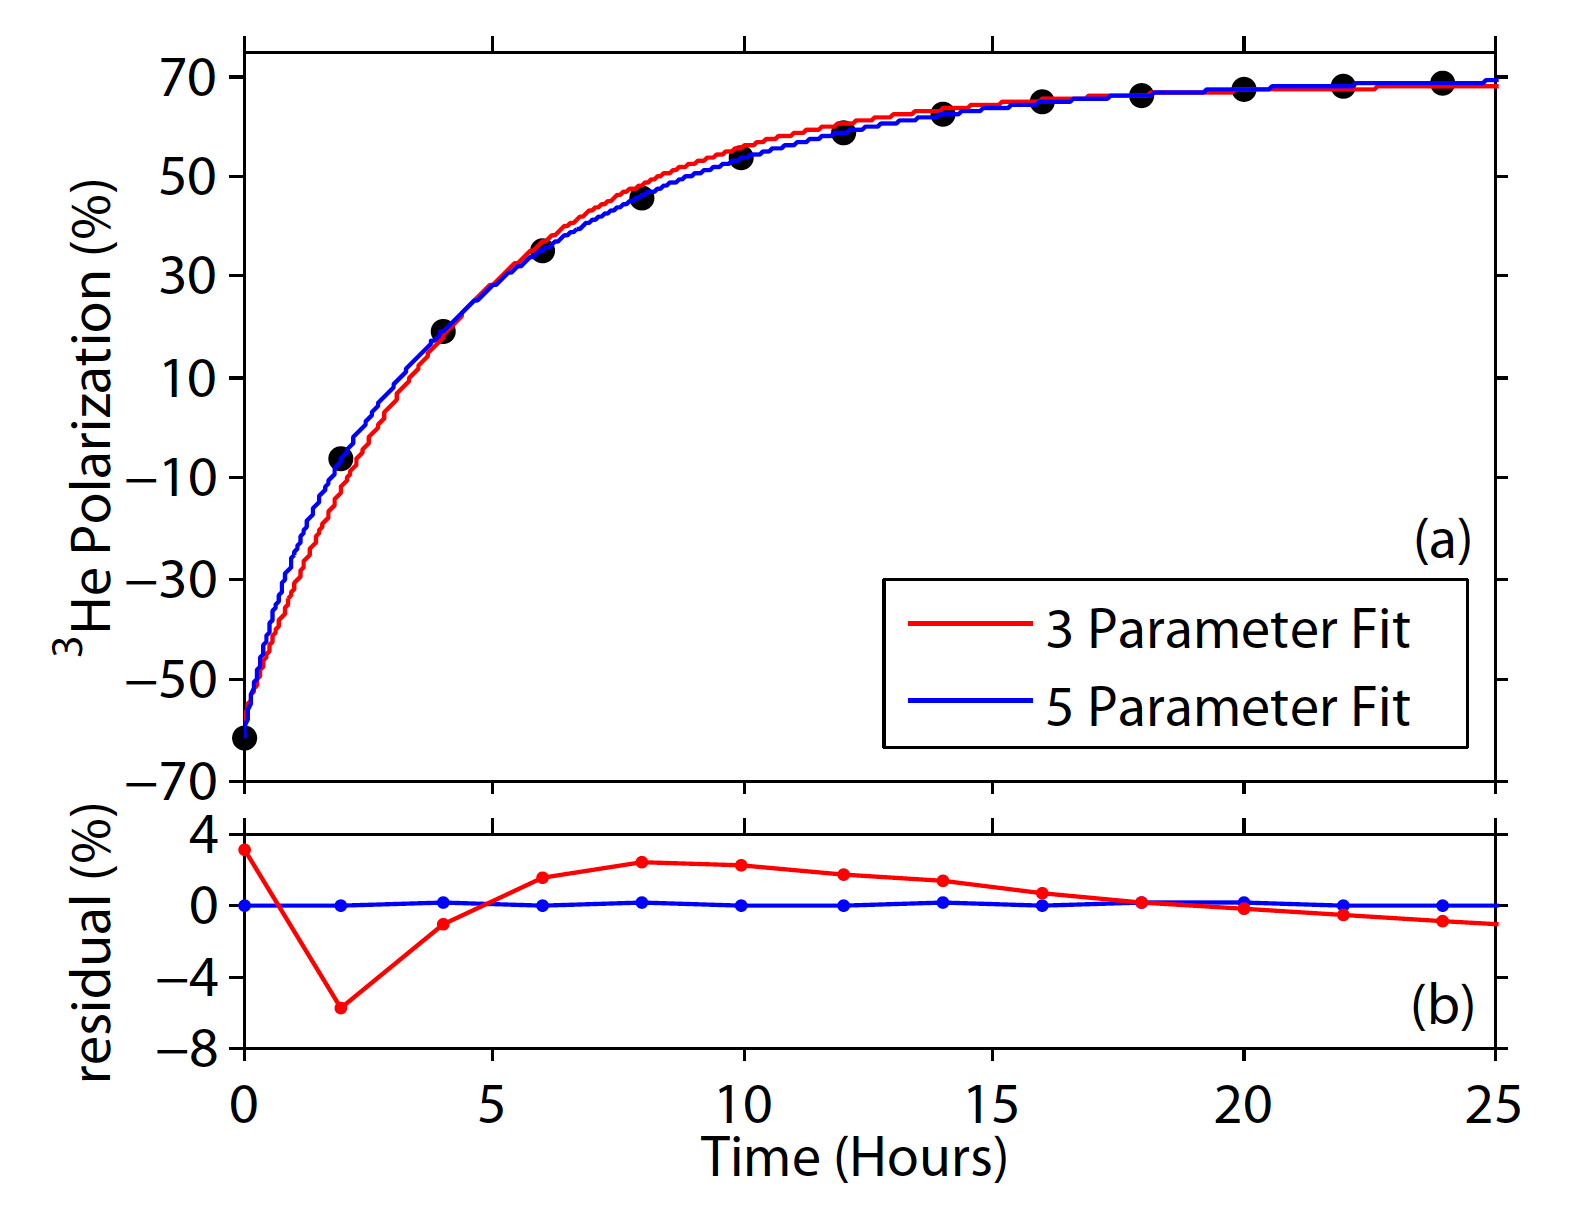
\includegraphics{Spinup.png}}
	\caption{{(a) Shown is a spinup of the target Brady. The spinup data has been fit with a 3-parameter and a 5-parameter formalism. (b) The residuals of the two fits. The error for 3-parameter fit is larger because it does not account for diffusion between two chambers. Adopted from~\cite{PhysRevC.91.055205}.}}
\end{figure}
	
The energy levels of $^{87}$Rb are shown in Fig.~\ref{fig:foms}.
where $\Gamma_{A}$ is the pressure dependent FWHM, $\Gamma_{A}\approx 0.04nm/amg \cdot [^{3}He]$.

\addcontentsline{toc}{chapter}{Bibliography}
\bibliography{ref}

\end{document}